\documentclass[border=10pt]{standalone}
\usepackage{tikz}
\usepackage{pgfplots}
\pgfplotsset{compat=1.18}
\usepackage{amsmath}
\usepackage[utf8]{inputenc}
\usepackage[OT1]{fontenc}

\definecolor{coral}{RGB}{208,90,48}
\definecolor{teal}{RGB}{15,110,86}
\definecolor{amber}{RGB}{239,159,39}
\definecolor{gray1}{RGB}{180,178,169}
\definecolor{dangerred}{RGB}{162,45,45}

\begin{document}
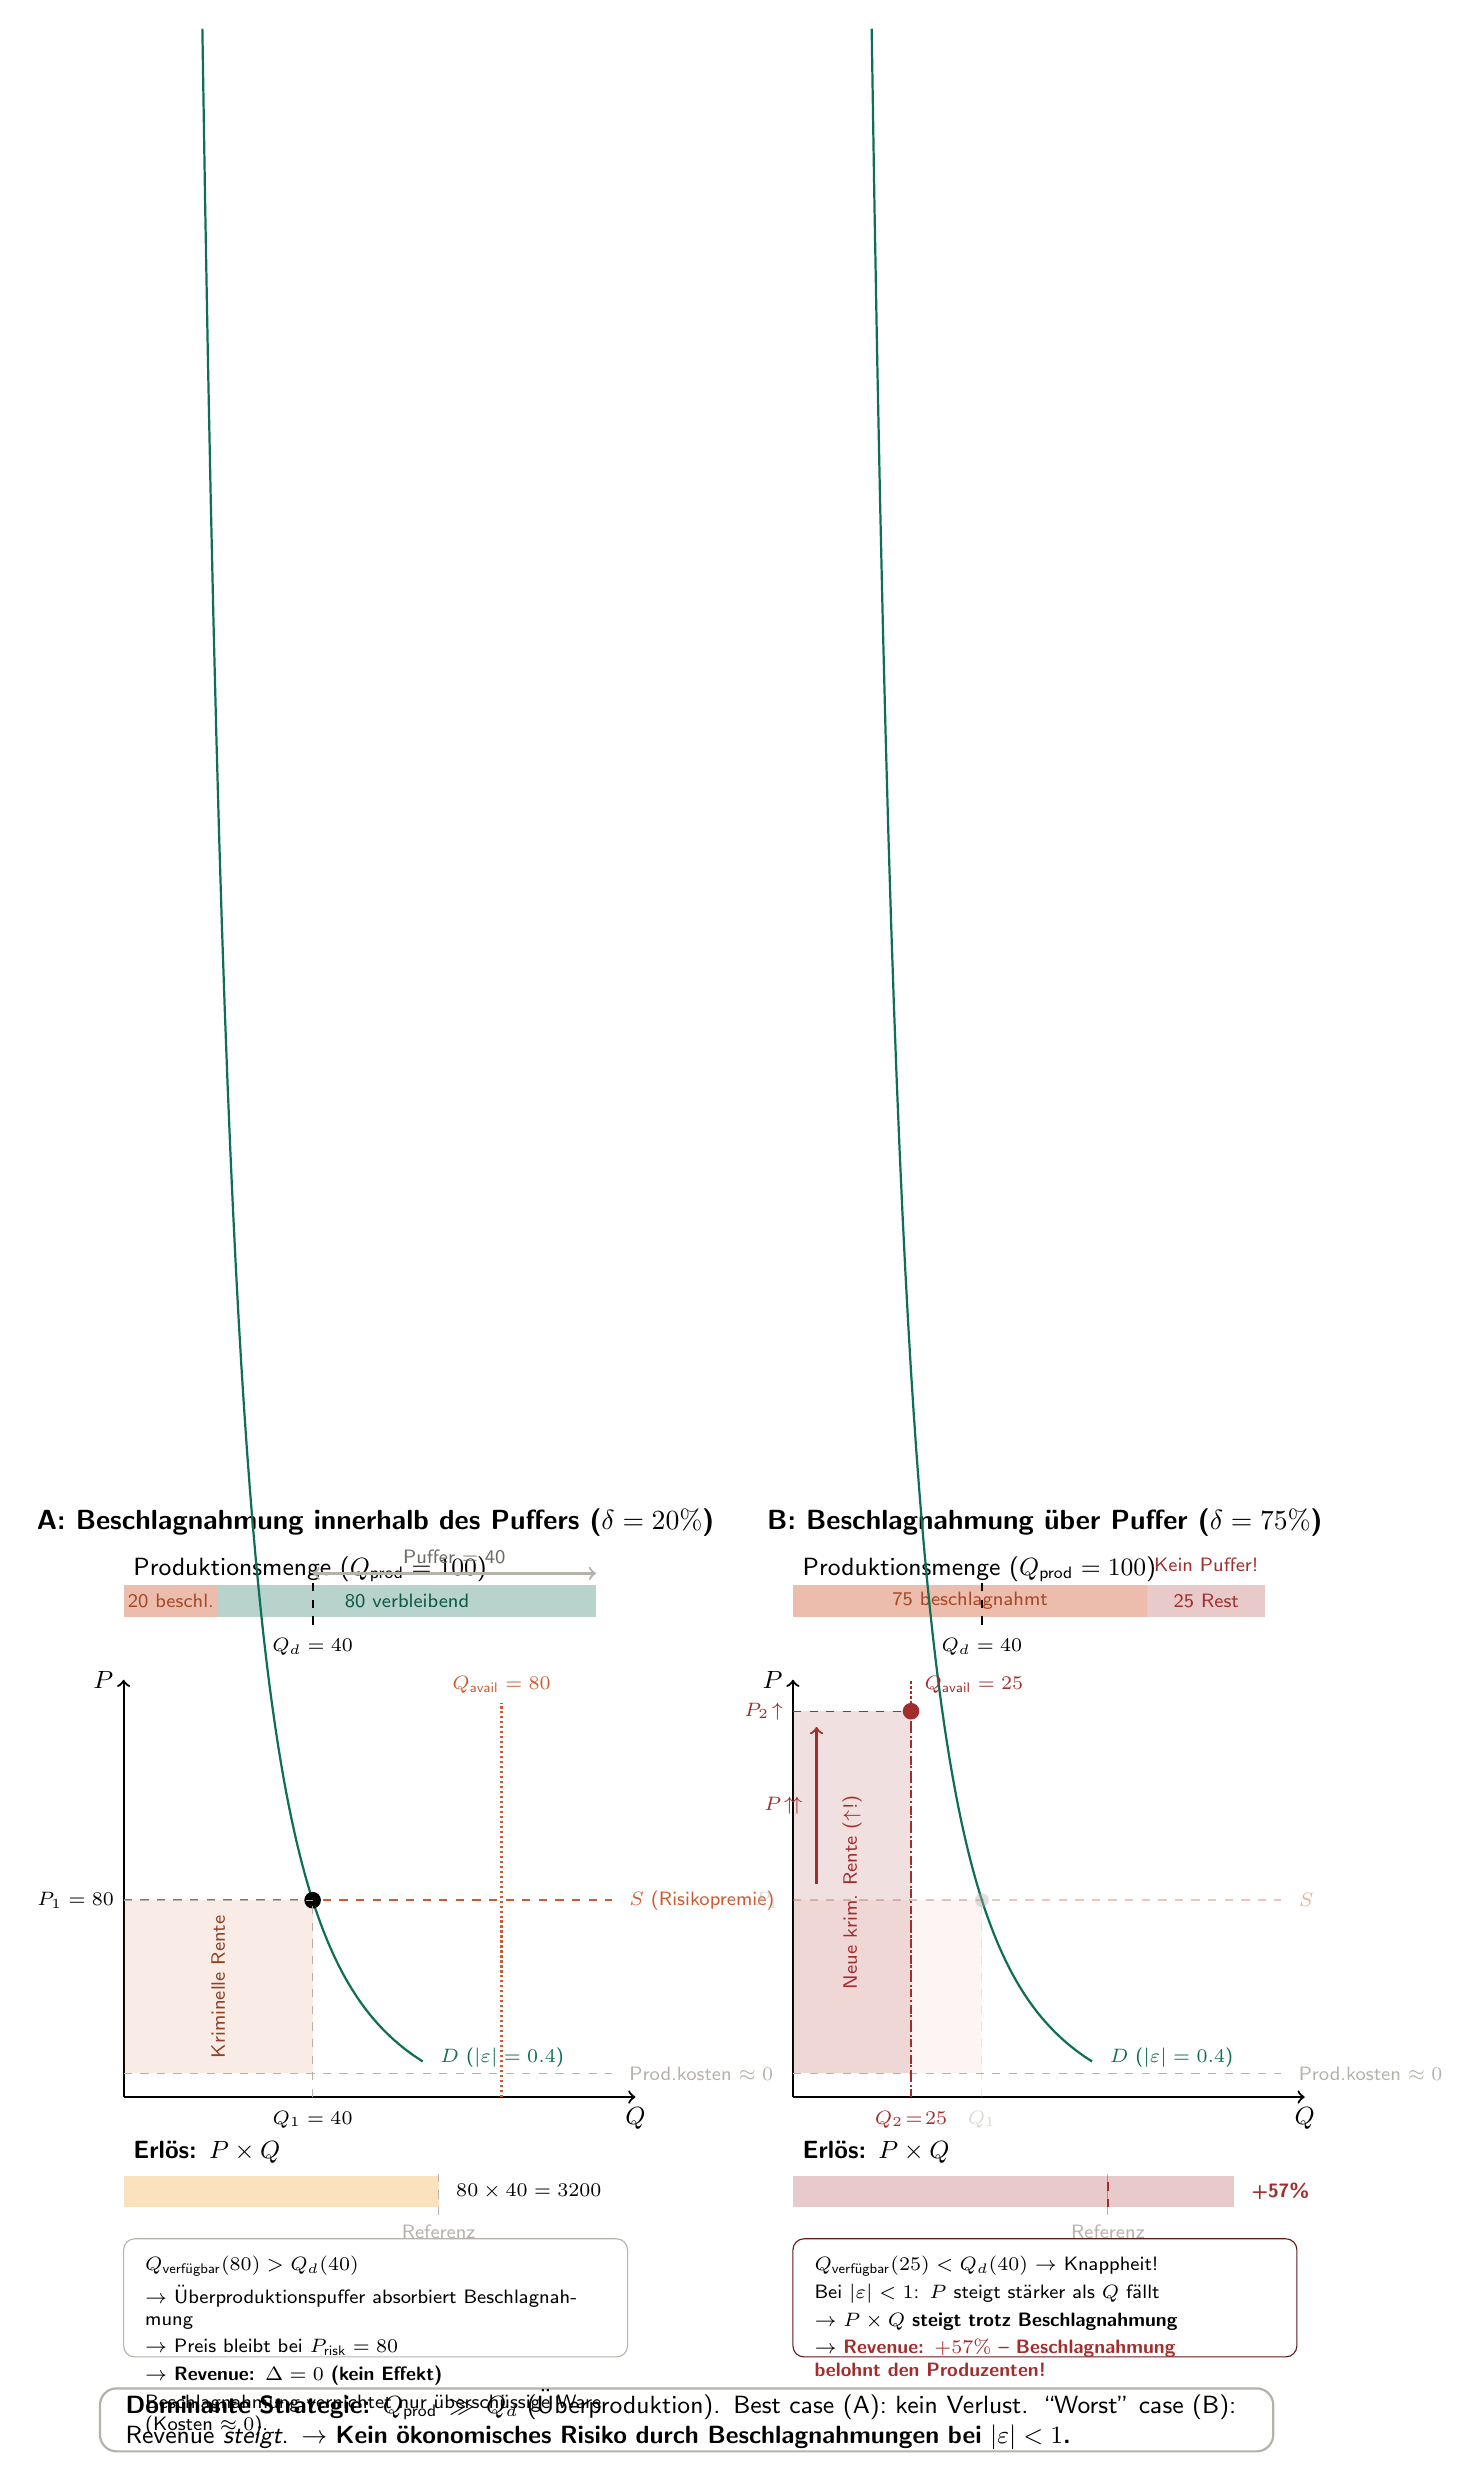
\begin{tikzpicture}

% ============================================================
% PANEL A: Seizure within buffer (delta = 20%)
% ============================================================
\begin{scope}[shift={(0,0)}]

  \node[font=\bfseries\sffamily] at (3.2,7.8) {A: Beschlagnahmung innerhalb des Puffers ($\delta = 20\%$)};

  % --- Production bar ---
  \node[font=\small\sffamily, anchor=west] at (0,7.2) {Produktionsmenge ($Q_{\text{prod}} = 100$)};

  % Seized
  \fill[coral, opacity=0.4] (0,6.6) rectangle (1.2,7.0);
  \node[font=\scriptsize\sffamily, coral!80!black] at (0.6,6.8) {20 beschl.};

  % Remaining
  \fill[teal, opacity=0.3] (1.2,6.6) rectangle (6.0,7.0);
  \node[font=\scriptsize\sffamily, teal!80!black] at (3.6,6.8) {80 verbleibend};

  % Demand threshold
  \draw[thick, dashed] (2.4,6.5) -- (2.4,7.1);
  \node[font=\scriptsize\sffamily, anchor=north] at (2.4,6.45) {$Q_d = 40$};

  % Buffer label
  \draw[<->, gray1, thick] (2.4,7.15) -- (6.0,7.15);
  \node[font=\scriptsize\sffamily, gray1!60!black, anchor=south] at (4.2,7.15) {Puffer = 40};

  % --- S/D Diagram ---
  % Axes
  \draw[->, thick] (0,0.5) -- (0,5.8) node[left, font=\small\sffamily] {$P$};
  \draw[->, thick] (0,0.5) -- (6.5,0.5) node[below, font=\small\sffamily] {$Q$};

  % Production costs ~ 0
  \draw[gray1, dashed, thin] (0,0.8) -- (6.2,0.8);
  \node[font=\scriptsize\sffamily, gray1, anchor=west] at (6.3,0.8) {Prod.kosten $\approx 0$};

  % S line (flat, risk premium)
  \draw[coral, thick, dashed] (0,3.0) -- (6.2,3.0);
  \node[font=\scriptsize\sffamily, coral, anchor=west] at (6.3,3.0) {$S$ (Risikopremie)};

  % Criminal rent rectangle
  \fill[coral, opacity=0.12] (0,0.8) rectangle (2.4,3.0);
  \node[font=\scriptsize\sffamily, coral!70!black, rotate=90] at (1.2,1.9) {Kriminelle Rente};

  % D curve (steep/inelastic), passing through (Q_d=40, P_risk=80)
  % Map: Q=40 -> x=2.4, P=80 -> y=3.0
  % Using P = P_risk * (Q_d/Q)^(1/epsilon), epsilon=0.4
  \draw[teal, thick, domain=1.0:3.8, samples=80] 
    plot ({\x}, {3.0 * (2.4/\x)^(2.5)});
  \node[font=\scriptsize\sffamily, teal, anchor=west] at (3.9,1.0) {$D$ ($|\varepsilon|=0.4$)};

  % Supply available line (vertical at Q_avail = 80 mapped, but we show Q_d intersection)
  % Q_avail > Q_d, so equilibrium is at Q_d on the flat S
  \draw[coral, thick, densely dotted] (4.8,0.5) -- (4.8,5.5);
  \node[font=\scriptsize\sffamily, coral, anchor=south] at (4.8,5.5) {$Q_{\text{avail}}=80$};

  % Equilibrium dot
  \fill (2.4,3.0) circle (3pt);

  % Dashed lines to axes
  \draw[gray1, dashed, thin] (0,3.0) -- (2.4,3.0);
  \draw[gray1, dashed, thin] (2.4,0.5) -- (2.4,3.0);
  \node[font=\scriptsize\sffamily, anchor=east] at (0,3.0) {$P_1=80$};
  \node[font=\scriptsize\sffamily, anchor=north] at (2.4,0.45) {$Q_1=40$};

  % Revenue bar
  \node[font=\small\sffamily\bfseries, anchor=west] at (0,-0.2) {Erl\"os: $P \times Q$};
  \fill[amber, opacity=0.3] (0,-0.9) rectangle (4.0,-0.5);
  \draw[gray1, dashed] (4.0,-1.0) -- (4.0,-0.4);
  \node[font=\scriptsize\sffamily, anchor=west] at (4.1,-0.7) {$80 \times 40 = 3200$};
  \node[font=\scriptsize\sffamily, gray1, anchor=north] at (4.0,-1.0) {Referenz};

  % Annotation box
  \draw[rounded corners=4pt, gray1] (0,-2.8) rectangle (6.4,-1.3);
  \node[font=\scriptsize\sffamily, anchor=north west, text width=6cm] at (0.15,-1.4) {%
    $Q_{\text{verf\"ugbar}} (80) > Q_d (40)$ \\[2pt]
    $\rightarrow$ \"Uberproduktionspuffer absorbiert Beschlagnahmung \\[2pt]
    $\rightarrow$ Preis bleibt bei $P_{\text{risk}} = 80$ \\[2pt]
    $\rightarrow$ \textbf{Revenue: $\Delta = 0$ (kein Effekt)} \\[2pt]
    Beschlagnahmung vernichtet nur \"ubersch\"ussige Ware (Kosten $\approx 0$).
  };

\end{scope}

% ============================================================
% PANEL B: Seizure exceeds buffer (delta = 75%)
% ============================================================
\begin{scope}[shift={(8.5,0)}]

  \node[font=\bfseries\sffamily] at (3.2,7.8) {B: Beschlagnahmung \"uber Puffer ($\delta = 75\%$)};

  % --- Production bar ---
  \node[font=\small\sffamily, anchor=west] at (0,7.2) {Produktionsmenge ($Q_{\text{prod}} = 100$)};

  % Seized
  \fill[coral, opacity=0.4] (0,6.6) rectangle (4.5,7.0);
  \node[font=\scriptsize\sffamily, coral!80!black] at (2.25,6.8) {75 beschlagnahmt};

  % Remaining
  \fill[dangerred, opacity=0.25] (4.5,6.6) rectangle (6.0,7.0);
  \node[font=\scriptsize\sffamily, dangerred] at (5.25,6.8) {25 Rest};

  % Demand threshold
  \draw[thick, dashed] (2.4,6.5) -- (2.4,7.1);
  \node[font=\scriptsize\sffamily, anchor=north] at (2.4,6.45) {$Q_d = 40$};

  % No buffer label
  \node[font=\scriptsize\sffamily, dangerred, anchor=south] at (5.25,7.05) {Kein Puffer!};

  % --- S/D Diagram ---
  % Axes
  \draw[->, thick] (0,0.5) -- (0,5.8) node[left, font=\small\sffamily] {$P$};
  \draw[->, thick] (0,0.5) -- (6.5,0.5) node[below, font=\small\sffamily] {$Q$};

  % Production costs ~ 0
  \draw[gray1, dashed, thin] (0,0.8) -- (6.2,0.8);
  \node[font=\scriptsize\sffamily, gray1, anchor=west] at (6.3,0.8) {Prod.kosten $\approx 0$};

  % S line (flat, risk premium) - now as reference
  \draw[coral, thick, dashed, opacity=0.35] (0,3.0) -- (6.2,3.0);
  \node[font=\scriptsize\sffamily, coral, opacity=0.5, anchor=west] at (6.3,3.0) {$S$};

  % Old criminal rent (reference, faded)
  \fill[coral, opacity=0.06] (0,0.8) rectangle (2.4,3.0);

  % New criminal rent (larger! P higher, Q lower but P*Q > old)
  % Q_avail = 25, mapped to x=1.5
  % P at Q=25: P = 80*(40/25)^(1/0.4) = 80*(1.6)^2.5 = 80*3.24 = 259
  % Mapped: P=259 -> y = 3.0/80*259 = 9.7... too high, let's scale
  % Better mapping: y = 0.8 + (P/80)*2.2, so P=80->y=3.0, P=200->y=6.3
  % P at Q=25: P = 80*(40/25)^2.5 = 80*3.24 = 259 -> y = 0.8+259/80*2.2 = 7.9 (clip)
  % Let's use P=200 for visual clarity (y=6.3)
  % Actually let me recalculate with gentler curve for visual fit
  % Use epsilon=0.5: P = 80*(40/Q)^2
  % At Q=25 (x=1.5): P = 80*(40/25)^2 = 80*2.56 = 204.8 -> y=0.8+204.8/80*2.2=6.44

  % New rent rectangle  
  \fill[dangerred, opacity=0.15] (0,0.8) rectangle (1.5,5.4);
  \node[font=\scriptsize\sffamily, dangerred, rotate=90] at (0.75,3.1) {Neue krim. Rente ($\uparrow$!)};

  % D curve (same as panel A)
  \draw[teal, thick, domain=1.0:3.8, samples=80] 
    plot ({\x}, {3.0 * (2.4/\x)^(2.5)});
  \node[font=\scriptsize\sffamily, teal, anchor=west] at (3.9,1.0) {$D$ ($|\varepsilon|=0.4$)};

  % Supply available line (vertical at Q_avail = 25, mapped to x=1.5)
  \draw[dangerred, thick, densely dotted] (1.5,0.5) -- (1.5,5.8);
  \node[font=\scriptsize\sffamily, dangerred, anchor=south west] at (1.55,5.5) {$Q_{\text{avail}}=25$};

  % New equilibrium: intersection of D and vertical Q_avail=25
  % P at x=1.5: y = 3.0*(2.4/1.5)^2.5 = 3.0*(1.6)^2.5 = 3.0*3.24 = 9.7 -> clipped
  % For visual: put equilibrium at y=5.4 (represents P~170)
  \fill[dangerred] (1.5,5.4) circle (3pt);

  % Old equilibrium (faded)
  \fill[gray1, opacity=0.4] (2.4,3.0) circle (2.5pt);

  % Dashed lines to axes (new)
  \draw[dangerred, dashed, thin] (0,5.4) -- (1.5,5.4);
  \draw[dangerred, dashed, thin] (1.5,0.5) -- (1.5,5.4);
  \node[font=\scriptsize\sffamily, dangerred, anchor=east] at (0,5.4) {$P_2 \!\uparrow$};
  \node[font=\scriptsize\sffamily, dangerred, anchor=north] at (1.5,0.45) {$Q_2\!=\!25$};

  % Old reference dashes
  \draw[gray1, dashed, thin, opacity=0.3] (0,3.0) -- (2.4,3.0);
  \draw[gray1, dashed, thin, opacity=0.3] (2.4,0.5) -- (2.4,3.0);
  \node[font=\scriptsize\sffamily, gray1, opacity=0.5, anchor=east] at (-0.05,3.0) {$P_1$};
  \node[font=\scriptsize\sffamily, gray1, opacity=0.5, anchor=north] at (2.4,0.45) {$Q_1$};

  % Arrow showing price increase
  \draw[->, thick, dangerred] (0.3,3.2) -- (0.3,5.2);
  \node[font=\scriptsize\sffamily, dangerred, anchor=east] at (0.25,4.2) {$P\!\uparrow\!\uparrow$};

  % Revenue bar (LARGER than reference!)
  \node[font=\small\sffamily\bfseries, anchor=west] at (0,-0.2) {Erl\"os: $P \times Q$};
  % Old reference
  \draw[gray1, dashed] (4.0,-1.0) -- (4.0,-0.4);
  \node[font=\scriptsize\sffamily, gray1, anchor=north] at (4.0,-1.0) {Referenz};
  % New revenue bar (longer! ~+60%)
  \fill[dangerred, opacity=0.25] (0,-0.9) rectangle (5.6,-0.5);
  \draw[dangerred, thick, dashed] (4.0,-0.9) -- (4.0,-0.5);
  \node[font=\scriptsize\sffamily, dangerred, anchor=west] at (5.7,-0.7) {\textbf{+57\%}};

  % Annotation box
  \draw[rounded corners=4pt, dangerred!60!black] (0,-2.8) rectangle (6.4,-1.3);
  \node[font=\scriptsize\sffamily, anchor=north west, text width=6cm] at (0.15,-1.4) {%
    $Q_{\text{verf\"ugbar}} (25) < Q_d (40)$ $\rightarrow$ Knappheit! \\[2pt]
    Bei $|\varepsilon| < 1$: $P$ steigt st\"arker als $Q$ f\"allt \\[2pt]
    $\rightarrow$ $P \times Q$ \textbf{steigt trotz Beschlagnahmung} \\[2pt]
    $\rightarrow$ \textcolor{dangerred}{\textbf{Revenue: $+57\%$ -- Beschlagnahmung}} \\
    \textcolor{dangerred}{\textbf{belohnt den Produzenten!}}
  };

\end{scope}

% ============================================================
% Bottom: Conclusion
% ============================================================
\draw[thick, gray1, rounded corners=6pt] (-0.3,-4.0) rectangle (14.6,-3.2);
\node[font=\small\sffamily, text width=14.5cm, anchor=west] at (-0.1,-3.6) {%
  \textbf{Dominante Strategie:} $Q_{\text{prod}} \gg Q_d$ (\"Uberproduktion). 
  Best case (A): kein Verlust. ``Worst'' case (B): Revenue \textit{steigt}. 
  $\rightarrow$ \textbf{Kein \"okonomisches Risiko durch Beschlagnahmungen bei $|\varepsilon| < 1$.}
};

\end{tikzpicture}
\end{document}